\section{Common Patterns and Insights From the Failure Cases}
\label{sec:common_pattern}

\subsection*{Common patterns in multi-controller failure cases}
Table.1 summarizes the failure cases we analyzed and reproduced in this paper. 10 failure cases are analyzed and 8 out of 10 are reproduced in Kubernetes cluster. KinD cluster was used for failure reproduction.

\paragraph*{Most of failure cases involves scheduling behavior} 7 out 10 failure cases are directly or indirectly associated with scheduler. Some failure cases does not even require multiple controllers, e.g., S3, S5, S7. Even two conflicted configurations within a scheduler controller can result in failure. Kubernetes is composed of numerous controllers and other system components. Notably the schduler is one of the most complicated controllers. In addition how complicated it is, there are two fundamental design choices of kube-scheduler causing these failures. First, kube-scheduler does not revisit its previous scheduling decision. Once it schedules a pod in a node, the pod will never be re-scheduled to another node unless it is forced by external events like node failure or node taint. Kube-scheduler tries best effort at the time of scheduling and hands off. Even if first placement met all scheduling requirements, it can be violated later by future events. In S6 case, when pods were scheduled, they were spread by default scheduler policy. However, placement becomes skewed when the third node goes into maintenance and all pods in the node are evicted and scheduled in other nodes. Even after the third node becomes alive and able to host pods, the scheduler will not fix the skewed placement. 

\paragraph*{Needs for middle layer tools}
As confirmed in the failure case study, Kubernetes currently does not have any type of system layer preventing or warning configurations violating safety or liveness property. It is intrinsically challenging for Kubernetes to support additionaly prevention layer of safety and liveness property. There are three reasons that positions it in fundamentally difficult problem. 
First, there is no way to express user's intent in the current Kubernetes version. Someone might say just implementing a new layer doing that particular job will solve the problem. However, it is not trivial in which way users should express their intents. Which format should new commands look like, which commands should be added, etc. On top of that, it is putting extra burden to users who needs to learn additional commands. Kubernetes configurations are already sufficiently complicated. 
Second, to avoid multi-controller problems at the first place, one possible rather blind solution is removing features that contributes to potentially contradictorial configurations existing in mutliple controllers. For example, MostAllocated config in scheduler and high node utilization plugin in descheduler are pursuing the opposite purpose. One is trying to do bin packing (placing pods in high utilization node) and the other is trying to evict pods from high utilization nodes, hoping them to be scheduled in low utilization node. We can circumvent this probable multi-controller confliction by deprecating high node utilization plugin in descheduler. The same goal can be fulfilled by appropriate pod spreading configuration in scheduler. Although they might represent the same goal in high level, it can never be exactly same. It is simply because the mechanisms they achieve it are different - one is schedule and the other is eviction. They are in charge of exclusive roles.
Third, the confliction does not manifest always by turning on those plugins. It also depends on the exact configurations like threshold for each setting. Deleting conflicted features is overkill since the presence of potential confliction does not always lead to problem as well as it is not appropriate solution since their functionalities are fundamentally different.
Our conclusion is a need for middle layer verification tool. It takes input of Kubernetes yaml config files as they are and outputs whether that certain combination of configurations contains potential multi-controller problems. This new middle layer tool cannot fix the problem automatically since it still is not able to figure out user's intent and it should not be designed to do that because it would be too complicated. The new layer execution should happen offline or at least should be run in background. In other words, ti should not be in the critical path that can hurt the performance of cluster management task. We do not know what the most suitable verification technique is for this problem. We leave it for future work.


\paragraph*{Reproduced in a small scale} The first common pattern is all of failure cases presented in this paper does not need large scale cluster to reproduce them. Maximum number of nodes and pods used for reproduction are 3 and 6 respectively. It implies that they are substances of large scale cluster. When building testing tool or verification program, this observation can be leveraged to help their algorithms to be more efficient by reducing search space it needs to explore.


\begin{figure*}[t]
    \centering
    \subfloat[\centering D1 - Deployment + Kubelet]{{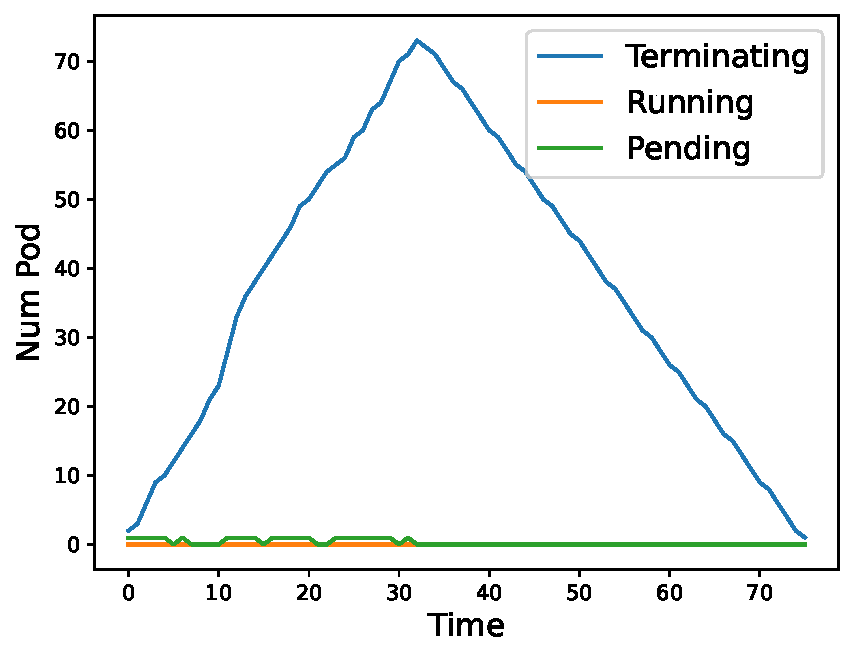
\includegraphics[width=0.5\columnwidth]{figure/num_pod-D1.pdf} }}%
    % \qquad
    \subfloat[\centering H1 - HPA + App CPU changes]{{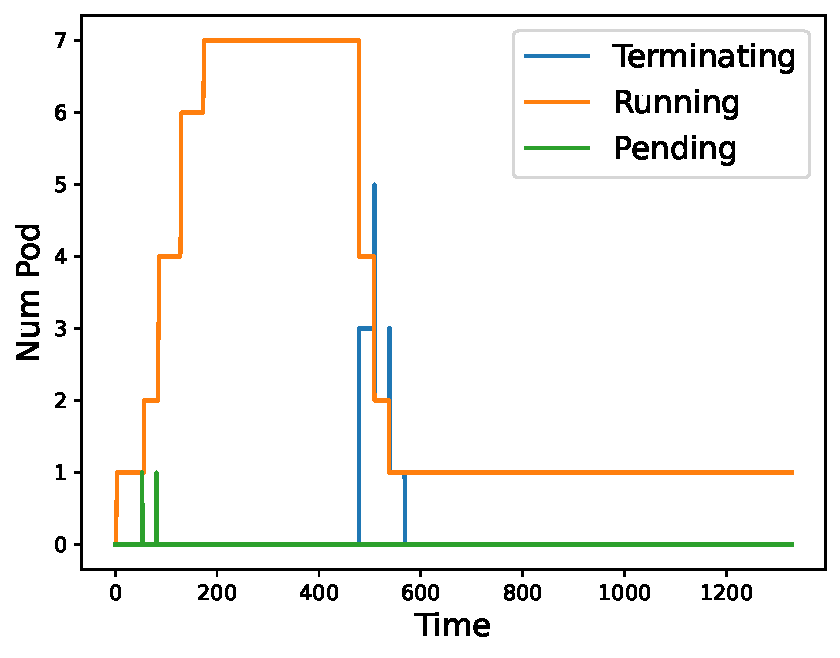
\includegraphics[width=0.5\columnwidth]{figure/num_pod-H1.pdf} }}%
    % \centering
    \subfloat[\centering S2 - Descheduler + Daemonset]{{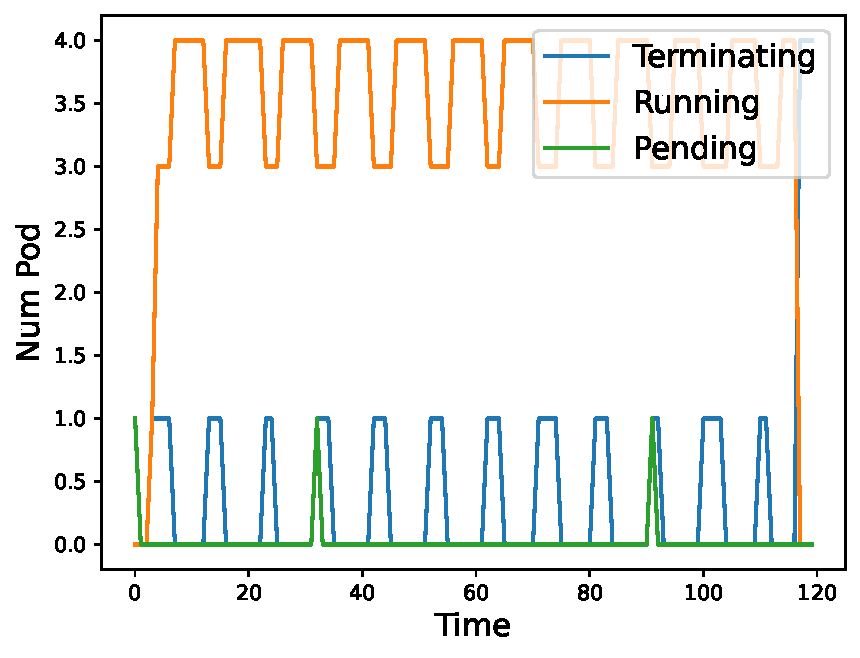
\includegraphics[width=0.5\columnwidth]{figure/num_pod-S2.pdf} }}%
    \subfloat[\centering S6 - Scheduler + Node maintenance]{{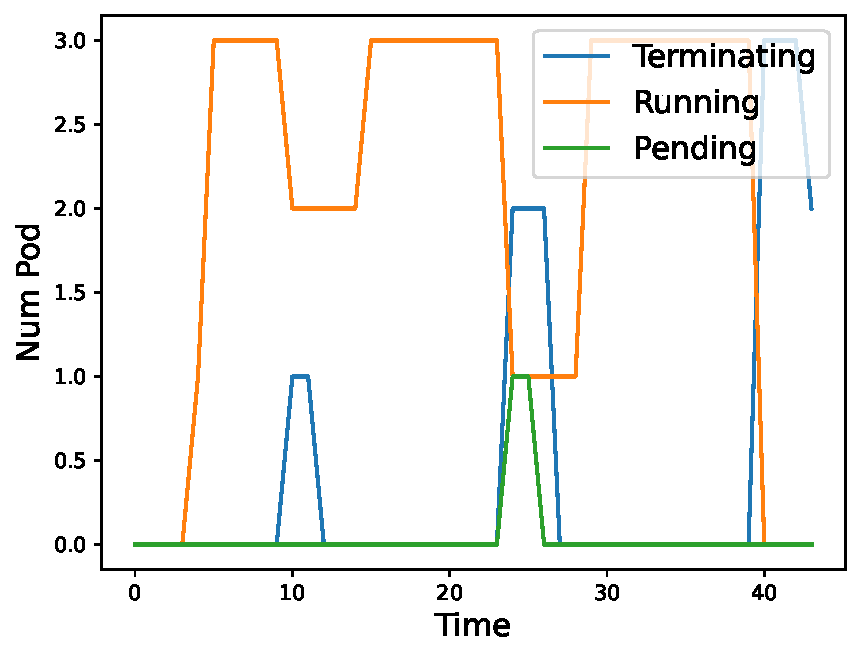
\includegraphics[width=0.5\columnwidth]{figure/num_pod-S6.pdf} }}%
    \caption{Number of pods over time for four failure cases.}
% \vspace{-20pt}
    \label{fig:num_pod}%
\end{figure*}